Tübingen hat keine Universität, Tübingen ist eine Universität. Daher existiert auch kein Uni-Campus im herkömmlichen Sinne, alles spielt sich irgendwo in der Stadt ab.
In eurem ersten Semester werdet ihr vor allem Vorlesung auf der Morgenstelle, im Kupferbau und im Psychologischen Institut haben. Für die letzten beiden haben wir leider noch keine Gebäudepläne, die wir hier abdrucken können.\\
In den höheren Semestern werdet ihr auch immer mal wieder Veranstaltungen auf dem Sand haben. Damit ihr euch dort zurechtfindet, haben wir hier ein paar Lagepläne zusammengefasst. Diese sind keinesfalls allumfassend, sie sollen euch lediglich eine grobe Orientierung durch den Dschungel der Uni-Gebäude bieten.
\subsection*{Morgenstelle}
\begin{figure}[ht!]
\centering
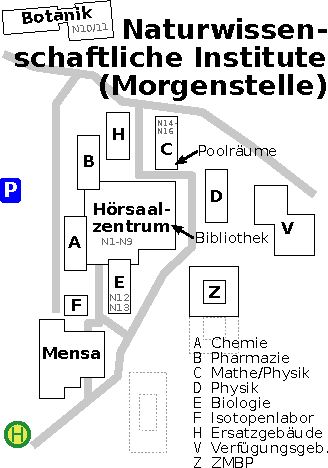
\includegraphics[width=0.5\textwidth]{kogni/anhang/lageplaene/uebersicht_morgenstelle.pdf}
\end{figure}
\newpage
\subsection*{Sand}
\begin{figure}[ht!]
	\centering
	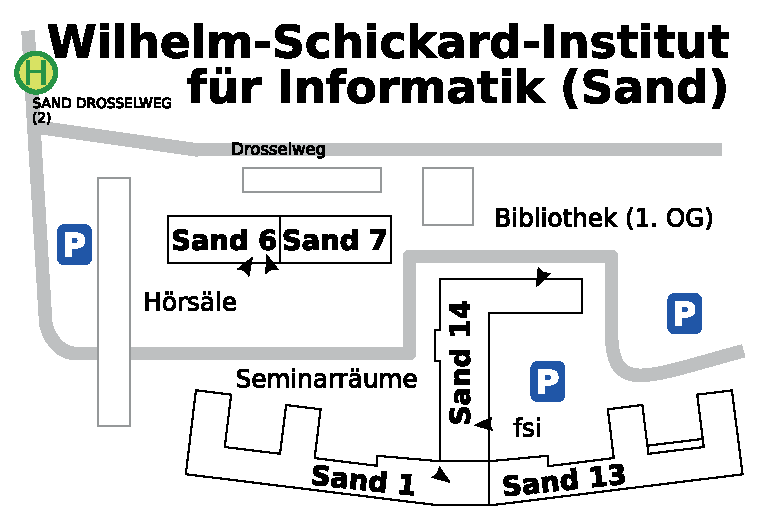
\includegraphics[width=0.8\textwidth]{kogni/anhang/lageplaene/uebersicht_sand.pdf}
\end{figure}
\subsection*{Psychologisches Institut}
\begin{figure}[ht!]
	\centering
	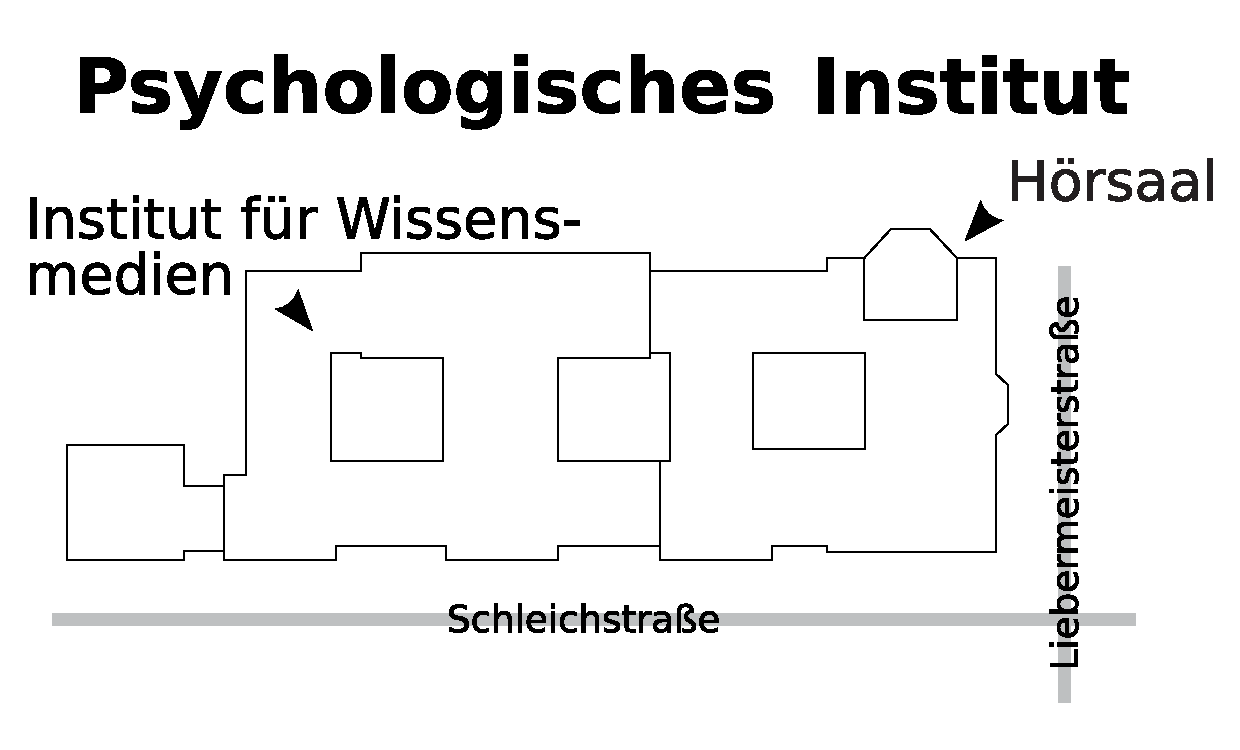
\includegraphics[width=\textwidth]{kogni/anhang/lageplaene/uebersicht_pi.pdf}
\end{figure}
%\newpage
%\subsubsection*{Sand, Erdgeschoss}~
%\begin{figure}[ht!]
%	\centering
%	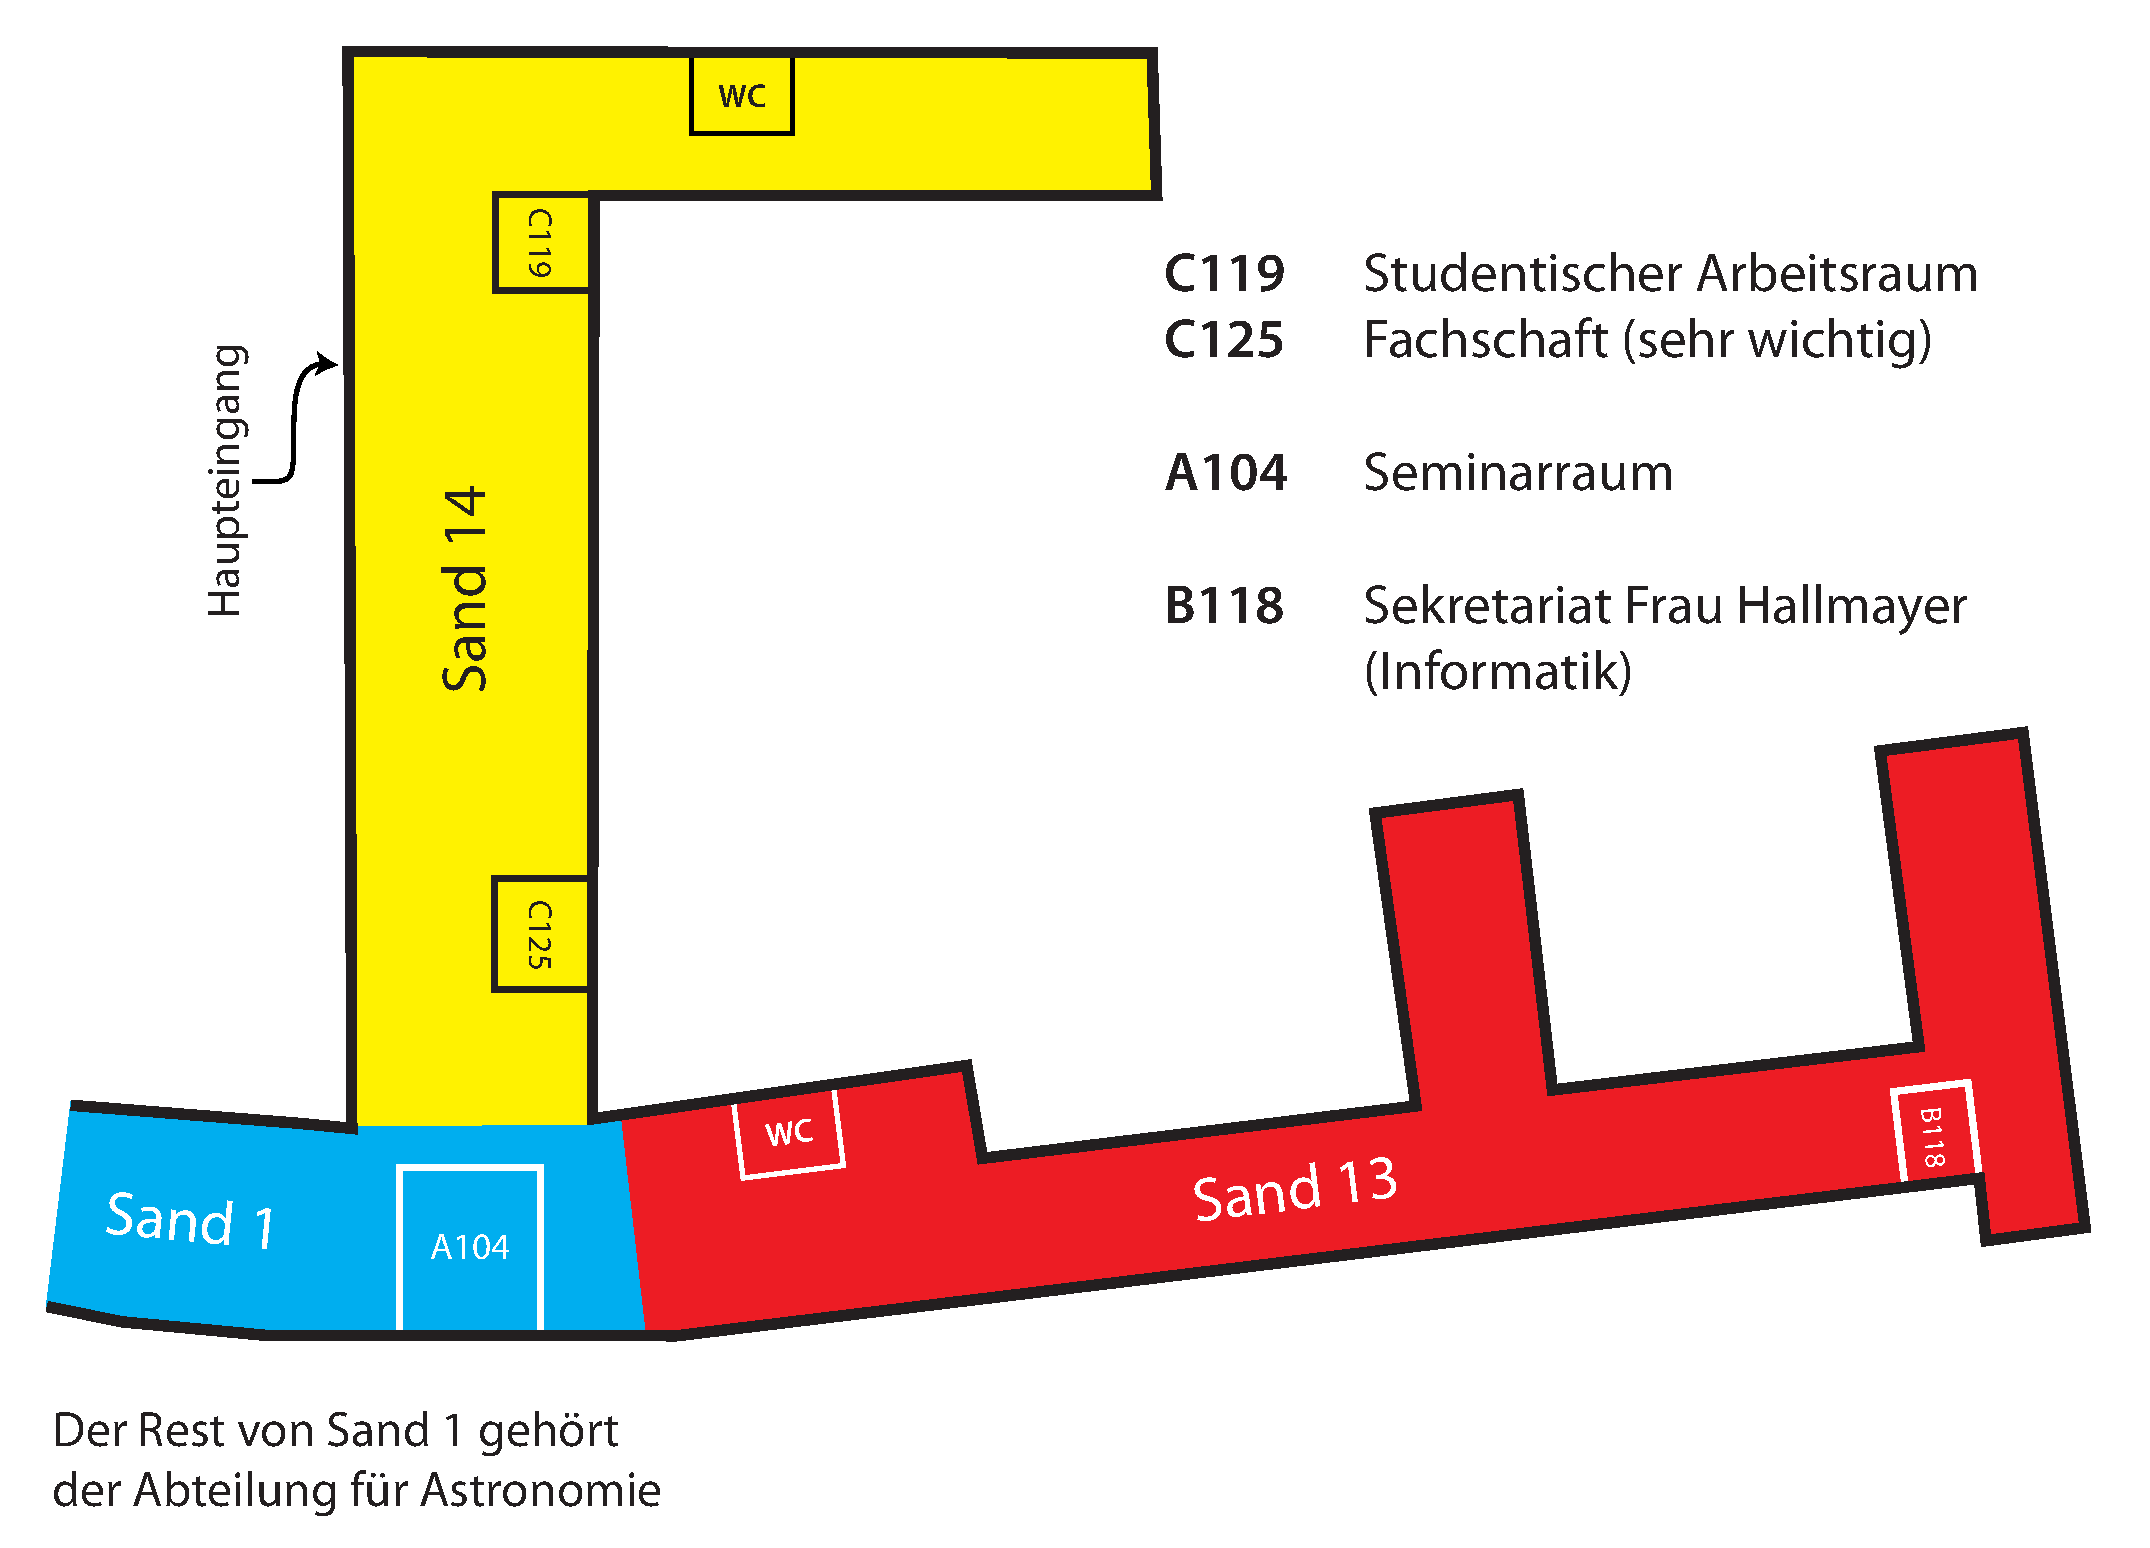
\includegraphics[width=0.8\textwidth]{anhang/lageplaene/sand_eg.pdf}
%\end{figure}
%\newpage 
%\subsubsection*{Sand, 1. OG}~
%\begin{figure}[ht!]
%	\centering
%	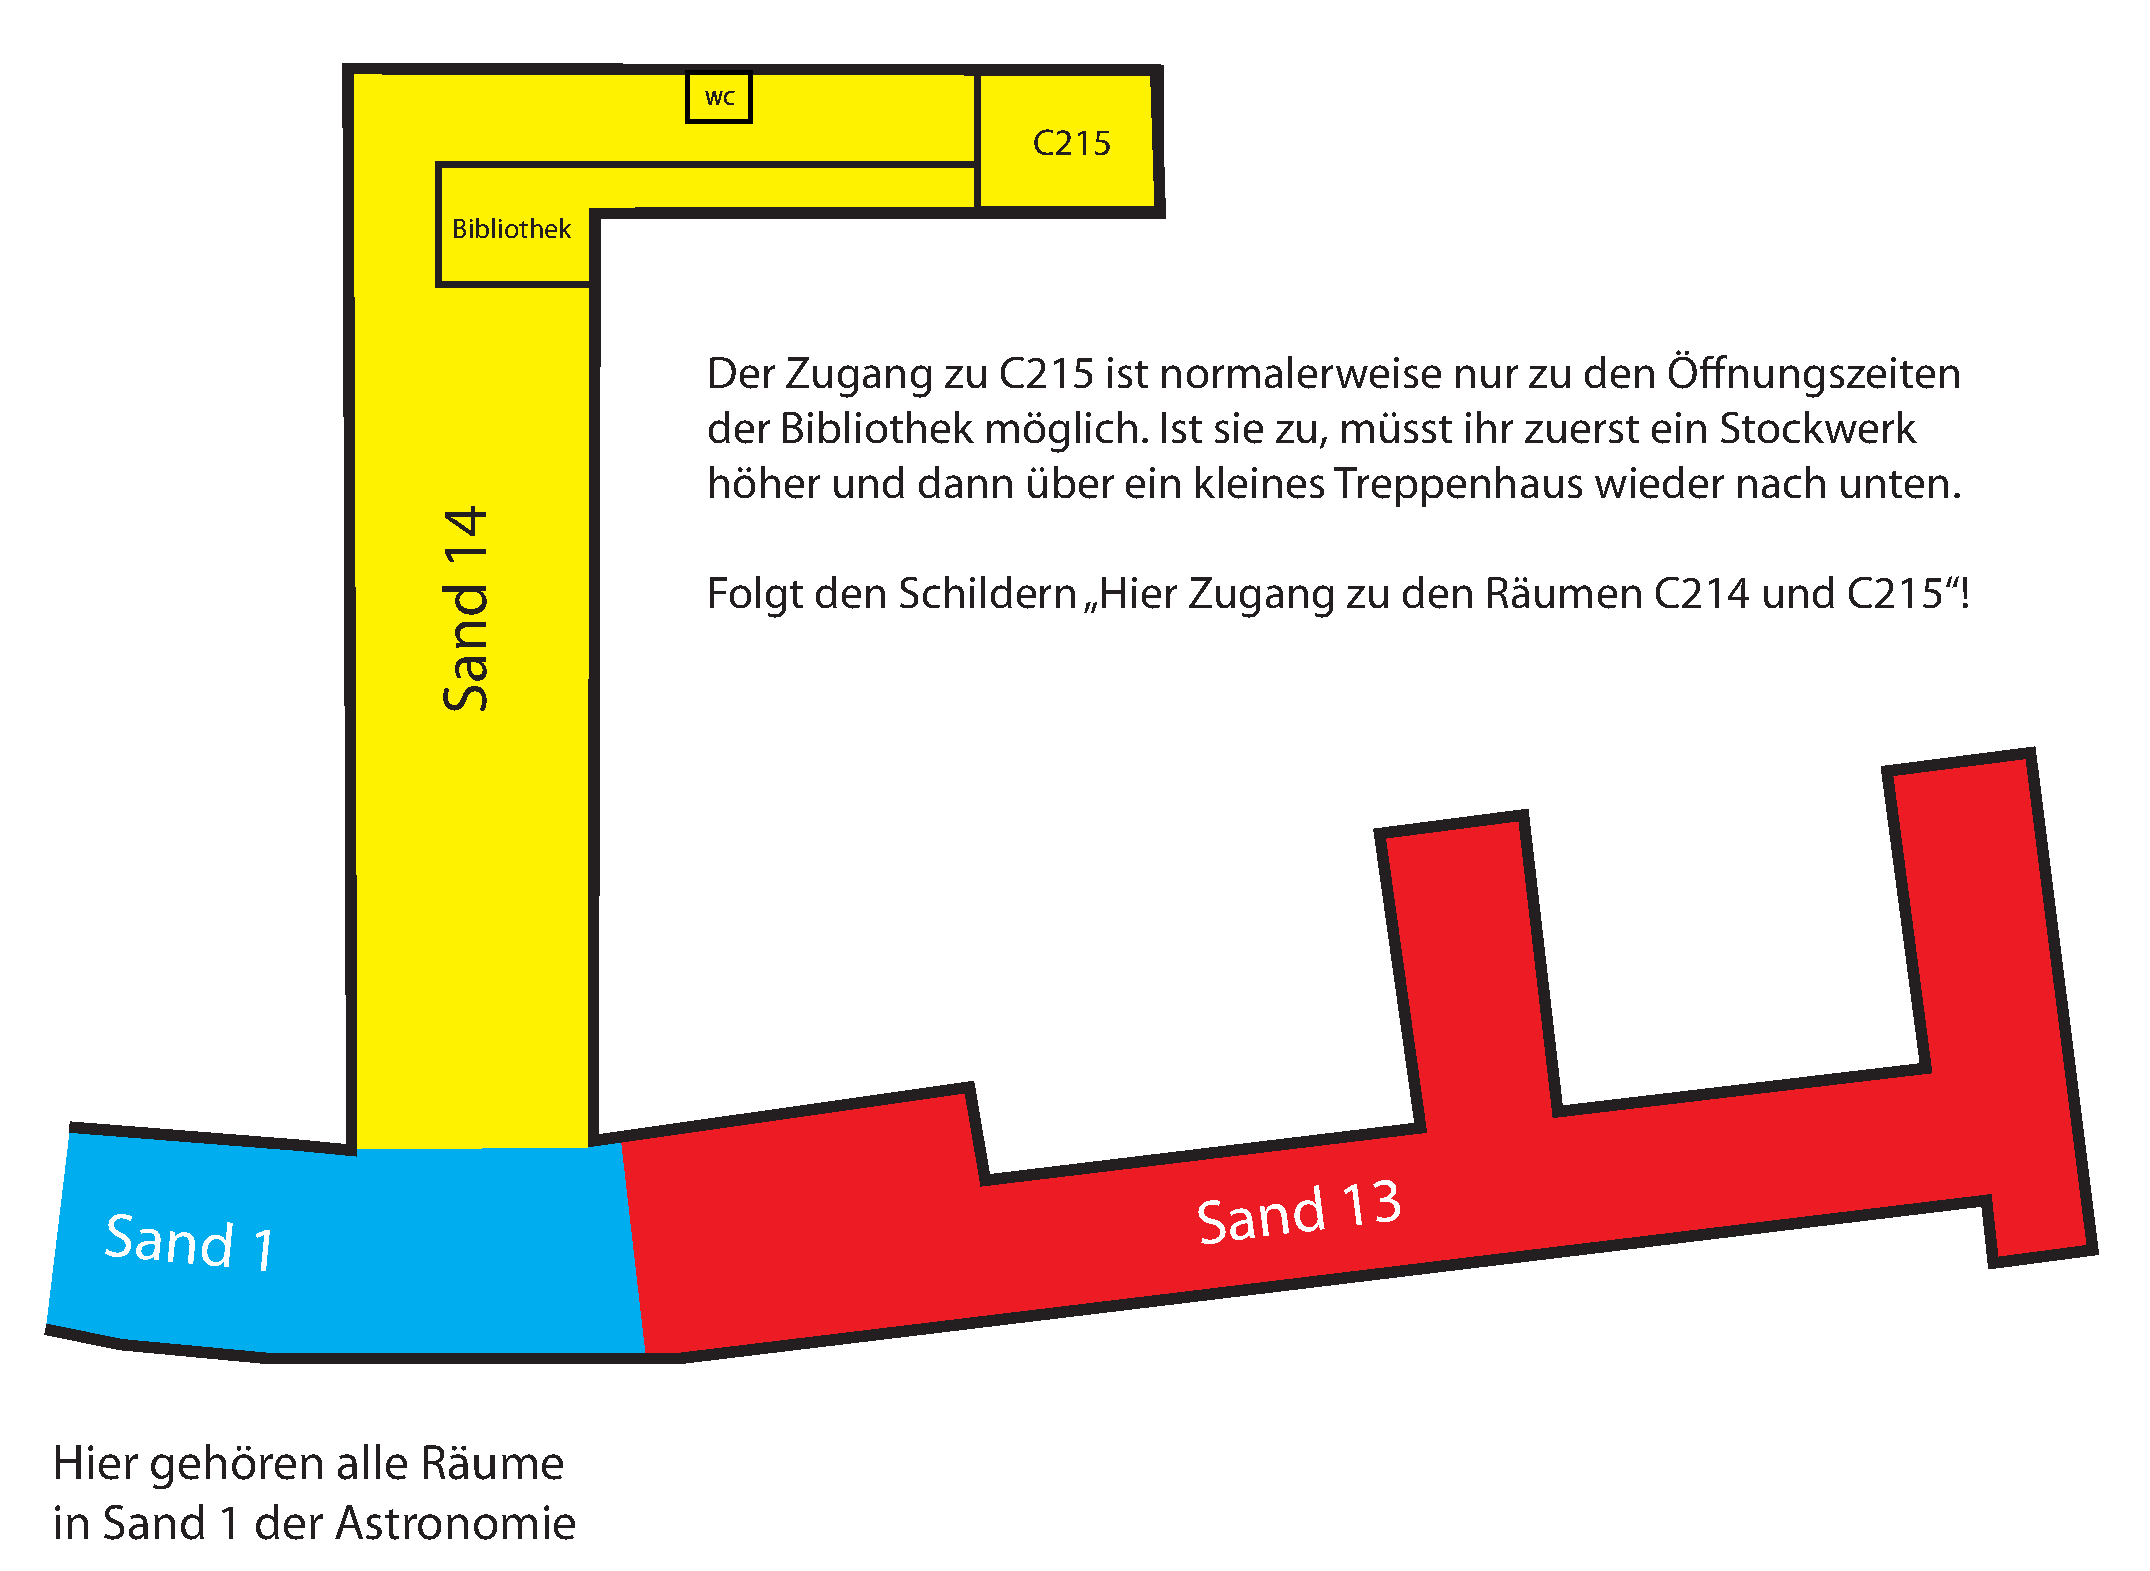
\includegraphics[width=0.8\textwidth]{anhang/lageplaene/sand_1og.pdf}
%\end{figure}
%\subsubsection*{Sand, 2. OG}~
%\begin{figure}[ht!]
%	\centering
%	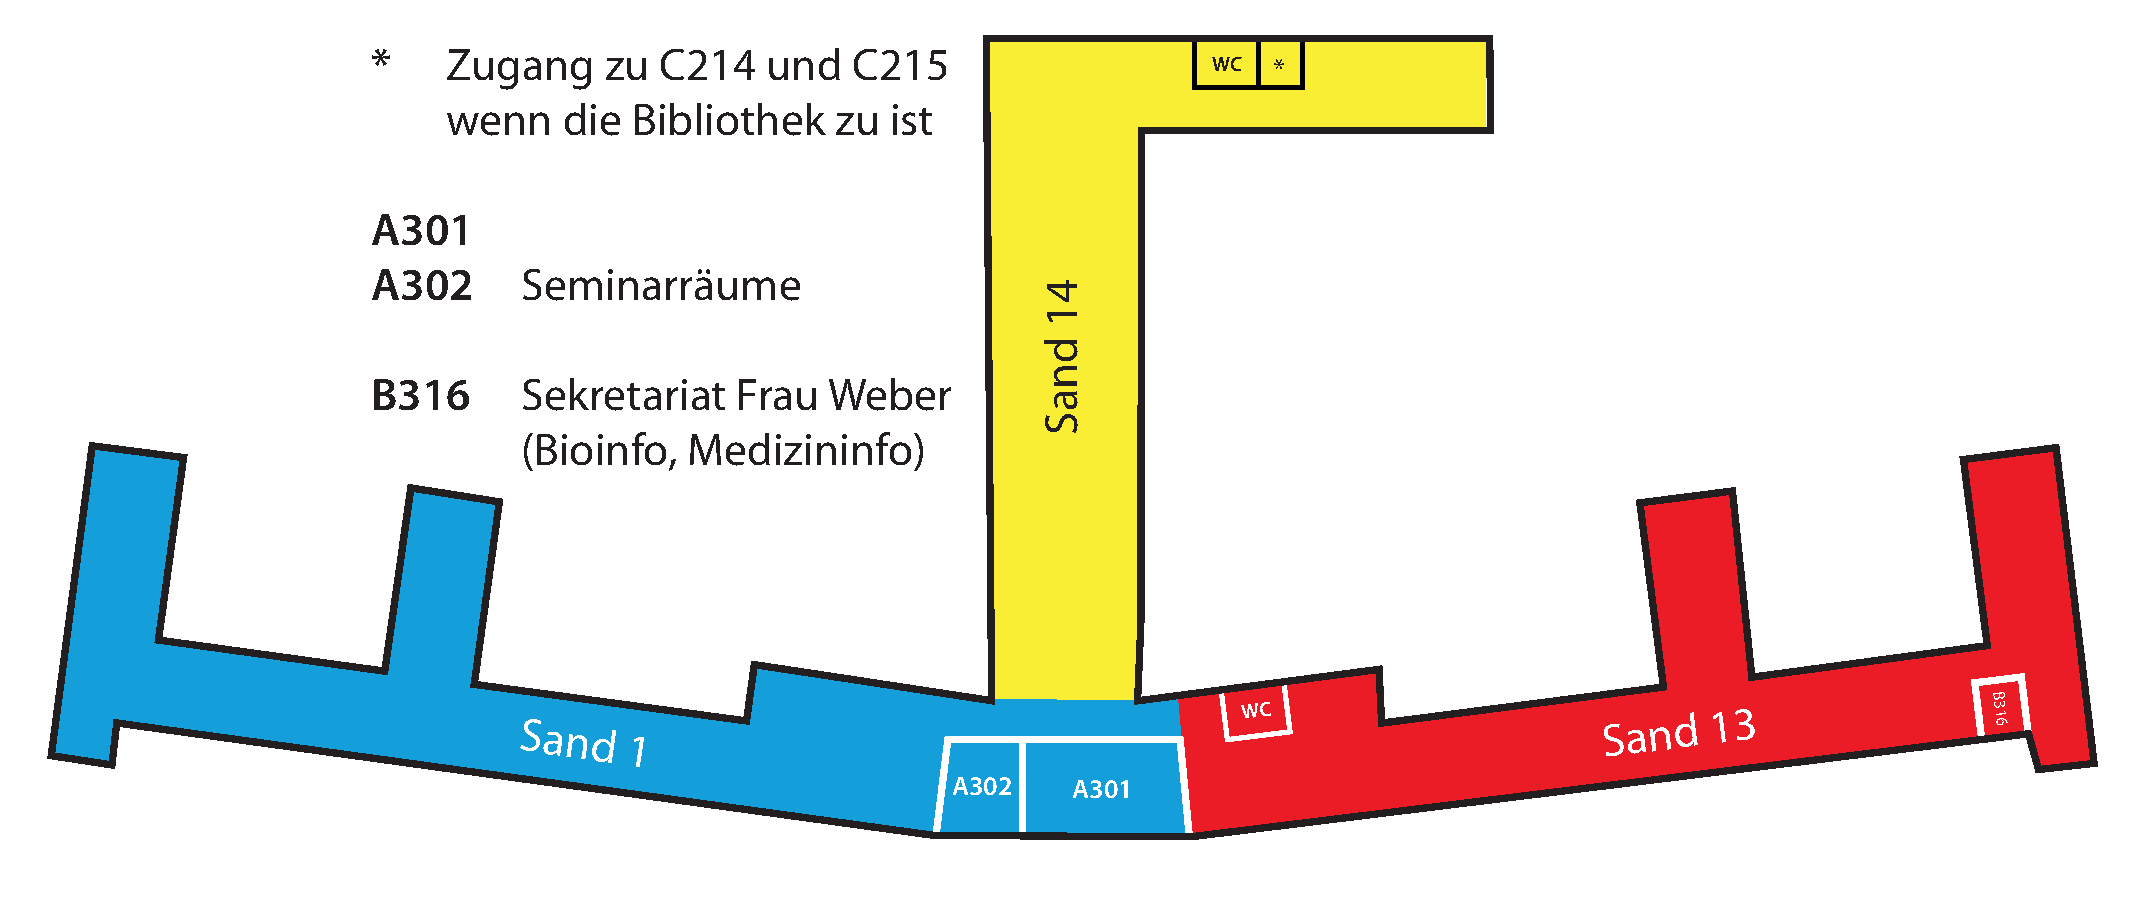
\includegraphics[width=\textwidth]{anhang/lageplaene/sand_2og.pdf}
%\end{figure}